\documentclass[
11pt, % The default document font size, options: 10pt, 11pt, 12pt
%codirector, % Uncomment to add a codirector to the title page
]{charter} 




% El títulos de la memoria, se usa en la carátula y se puede usar el cualquier lugar del documento con el comando \ttitle
\titulo{Sistema de monitoreo para un bioterio} 

% Nombre del posgrado, se usa en la carátula y se puede usar el cualquier lugar del documento con el comando \degreename
%\posgrado{Carrera de Especialización en Sistemas Embebidos} 
\posgrado{Carrera de Especialización en Internet de las Cosas} 
%\posgrado{Carrera de Especialización en Intelegencia Artificial}
%\posgrado{Maestría en Sistemas Embebidos} 
%\posgrado{Maestría en Internet de las cosas}

% Tu nombre, se puede usar el cualquier lugar del documento con el comando \authorname
\autor{LSI Norberto Antonio Rodríguez} 

% El nombre del director y co-director, se puede usar el cualquier lugar del documento con el comando \supname y \cosupname y \pertesupname y \pertecosupname
\director{Nombre del Director}
\pertenenciaDirector{pertenencia} 
% FIXME:NO IMPLEMENTADO EL CODIRECTOR ni su pertenencia
%\codirector{John Doe} % para que aparezca en la portada se debe descomentar la opción codirector en el documentclass
%\pertenenciaCoDirector{FIUBA}
\codirector{Nombre del Codirector} % para que aparezca en la portada se debe descomentar la opción codirector en el documentclass
\pertenenciaCoDirector{pertenencia}

% Nombre del cliente, quien va a aprobar los resultados del proyecto, se puede usar con el comando \clientename y \empclientename
\cliente{Dr. Juan Rosa}
\empresaCliente{Instituto de Medicina Regional - UNNE}

% Nombre y pertenencia de los jurados, se pueden usar el cualquier lugar del documento con el comando \jurunoname, \jurdosname y \jurtresname y \perteunoname, \pertedosname y \pertetresname.
\juradoUno{Nombre y Apellido (1)}
\pertenenciaJurUno{pertenencia (1)} 
\juradoDos{Nombre y Apellido (2)}
\pertenenciaJurDos{pertenencia (2)}
\juradoTres{Nombre y Apellido (3)}
\pertenenciaJurTres{pertenencia (3)}
 
\fechaINICIO{21 de junio de 2022}		%Fecha de inicio de la cursada de GdP \fechaInicioName
\fechaFINALPlan{16 de agosto de 2022} 	%Fecha de final de cursada de GdP
\fechaFINALTrabajo{15 de mayo de 2023}	%Fecha de defensa pública del trabajo final


\begin{document}

\maketitle
\thispagestyle{empty}
\pagebreak


\thispagestyle{empty}
{\setlength{\parskip}{0pt}
\tableofcontents{}
}
\pagebreak


\section*{Registros de cambios}
\label{sec:registro}


\begin{table}[ht]
\label{tab:registro}
\centering
\begin{tabularx}{\linewidth}{@{}|c|X|c|@{}}
\hline
\rowcolor[HTML]{C0C0C0} 
Revisión & \multicolumn{1}{c|}{\cellcolor[HTML]{C0C0C0}Detalles de los cambios realizados} & Fecha      \\ \hline
0      & Creación del documento.                                 &\fechaInicioName \\ \hline
1      & Se completa hasta el punto 5 inclusive.                 & 3 de julio de 2022 \\ \hline
2      & Se realizaron correcciones en distintos capítulos y se completó hasta el punto 9 inclusive.      & 9 de julio de 2022 \\ \hline
3      & Se realizaron correcciones en distintos capítulos y se completó hasta el punto 12 inclusive.      & 24 de julio de 2022 \\ \hline

%2      & Se completa hasta el punto 7 inclusive
%		  Se puede agregar algo más \newline
%		  En distintas líneas \newline
%		  Así                                                    & dd/mm/aaaa \\ \hline
%3      & Se completa hasta el punto 11 inclusive                & dd/mm/aaaa \\ \hline
%4      & Se completa el plan	                                 & dd/mm/aaaa \\ \hline
\end{tabularx}
\end{table}

\pagebreak



\section*{Acta de constitución del proyecto}
\label{sec:acta}

\begin{flushright}
Buenos Aires, \fechaInicioName
\end{flushright}

\vspace{2cm}

%Por medio de la presente se acuerda con el Lic. \authorname\hspace{1px} que su Trabajo Final de la \degreename\hspace{1px} se titulará ``\ttitle'', consistirá esencialmente en \textcolor{red}{la implementación de un prototipo de un sistema de monitoreo de las condiciones ambientales de un bioterio}, y tendrá un presupuesto preliminar estimado de \textcolor{red}{600} hs de trabajo y \textcolor{red}{\$75.000}, con fecha de inicio \fechaInicioName\hspace{1px} y fecha de presentación pública \fechaFinalName.%

Por medio de la presente se acuerda con el Lic. \authorname\hspace{1px} que su Trabajo Final de la \degreename\hspace{1px} se titulará ``\ttitle'', consistirá esencialmente en {la implementación de un prototipo de un sistema de monitoreo de las condiciones ambientales de un bioterio}, y tendrá un presupuesto preliminar estimado de {600} hs de trabajo y {ARS 1.002.977}, con fecha de inicio \fechaInicioName\hspace{1px} y fecha de presentación pública \fechaFinalName.

Se adjunta a esta acta la planificación inicial.

\vfill

% Esta parte se construye sola con la información que hayan cargado en el preámbulo del documento y no debe modificarla
\begin{table}[ht]
\centering
\begin{tabular}{ccc}
\begin{tabular}[c]{@{}c@{}}Dr. Ing. Ariel Lutenberg \\ Director posgrado FIUBA\end{tabular} & \hspace{2cm} & \begin{tabular}[c]{@{}c@{}}\clientename \\ \empclientename \end{tabular} \vspace{2.5cm} \\ 
\multicolumn{3}{c}{\begin{tabular}[c]{@{}c@{}} \supname \\ Director del Trabajo Final\end{tabular}} \vspace{2.5cm} \\
%\begin{tabular}[c]{@{}c@{}}\jurunoname \\ Jurado del Trabajo Final\end{tabular}     &  & \begin{tabular}[c]{@{}c@{}}\jurdosname\\ Jurado del Trabajo Final\end{tabular}  \vspace{2.5cm}  \\
%\multicolumn{3}{c}{\begin{tabular}[c]{@{}c@{}} \jurtresname\\ Jurado del Trabajo Final\end{tabular}} \vspace{.5cm}                                                                     
\end{tabular}
\end{table}




\section{1. Descripción técnica-conceptual del proyecto a realizar}
\label{sec:descripcion}

Un bioterio es un área artificial controlada donde se alojan animales o plantas bajo ciertas condiciones que permitan el desarrollo de la especie para guarda, crio o fines experimentales. Se deben registrar y estudiar las variables ambientales del laboratorio en general y de los bioterios en particular. Estas variables son: temperatura, humedad, cantidad de luz y CO2.

Estas áreas artificiales pueden utilizarse en nuevas disciplinas, por ejemplo, la ecoepidemiología, la cual supone un enfoque actual integrador del estudio de las enfermedades transmitidas a los animales, vegetales y humanos. Involucra los aspectos ecológicos y epidemiológicos denominados ecoepidemiológicos.

En el bioterio se tendrán artrópodos. Son animales invertebrados que actúan como uno de los agentes transmisores de enfermedades. Lo hacen por acción directa como vector o indirecta por acción traumática e irritante de su picadura. Este proceso es independiente a su rol en el ciclo de vida del agente etiológico viral, bacteriano o parasitario.

Los ciclos reproductivos de los artrópodos juegan un papel fundamental en la epidemiología de las enfermedades transmisibles. Hay diferentes causas que pueden afectar la transmisión de una enfermedad: las tasas de fecundidad y de mortalidad, la densidad de la población, su distribución por edades, la variación genética y la tasa de migración.  Algunas de estas variables pueden ser controladas en condiciones experimentales como la temperatura, humedad, ciclos de luz y ventilación como factores abióticos esenciales. Los ambientes especialmente diseñados, denominados insectarios, bioterios o animalarios, son la base de diversos estudios (Insect Morphology and Phylogeny, 2014).

Los artrópodos tienen varios estados en su ciclo de vida que están relacionados con su metamorfosis. La misma puede ser completa (holometábolos): huevo, larva, pupa e imago. O bien incompleta (hemimetábolos) huevos, ninfas, imagos y con clasificaciones intermedias.  Cada uno de los estados tienen requerimientos de temperatura, humedad o inundación.  

Los artrópodos hematófagos presentan limitaciones al momento de mantenerlos o de desarrollar su biología. Dependen primero, de la fuente de alimentación sanguínea y otros nutrientes.  También influye el rango de temperatura, que en general oscila entre 24-26 ºC y 80-95 \% de humedad relativa, con fotoperíodos mediante ciclos de luz-oscuridad de 12 horas e intensidad de luz y tipo de luz variable según requerimientos (Arthropod Containment Guidelines, 2019).

Otro factor importante a tener en cuenta con los artrópodos es que algunos requieren agua como parte del ciclo de vida; como los culícidos (mosquitos), simúlidos y ceratopogónidos (carachai, jejenes y polvorines). Todos dependen de la calidad del agua y la temperatura ambiente. A mayor temperatura el ciclo se acorta y, por el contrario, a menor temperatura se prolonga; algunos casos incluso entran en latencia (diapausa).

Las larvas pueden ser acuáticas o terrestres. Se deben considerar la humedad relativa ambiental y requerimientos nutricionales diferentes. En el caso de las pupas o crisálidas, dependiendo de la especie de vectores, la temperatura es importante debido a que es un estado de transformación y no de alimentación como en la anterior. Los imagos eclosionarán en un ambiente controlado, pero no significa que continúen el ciclo de reproducción y generen colonias parentales o bien filiales de la misma especie (Insect Morphology and Phylogeny, 2014).

El estudio de la biología en condiciones experimentales solo puede aplicarse a determinados artrópodos debido a las limitaciones propias del ciclo natural según experiencias preliminares.  Los resultados de estas observaciones permiten investigar aspectos referentes a los mecanismos de transmisión de patógenos, las comparaciones genéticas de poblaciones, la sistemática y la susceptibilidad a los insecticidas, entre otros. Sin embargo, existe gran dificultad de mantener a la mayoría de las colonias durante más de unas pocas generaciones lo que impide contar con tablas de vida. Esta situación limita la comprensión del comportamiento de las colonias en la naturaleza (Insect Morphology and Phylogeny, 2014).

El entorno de una colonia no puede duplicar las condiciones de nutrición, temperatura y humedad. La consecuencia será la afectación en el comportamiento de los adultos, la mortalidad de los huevos, el período de crecimiento de las larvas y la mortalidad de los adultos. No obstante, los datos de laboratorio proporcionan información de referencia esencial sobre el potencial reproductivo de algunas especies sometidas a experiencia como mosquitos y flebótomos (Diptera: Psychodidae: Phlebotominae). 

Para estudios en biología de poblaciones de flebótomos en el campo, estas observaciones proporcionan pautas para aproximar los límites de los comportamientos biológicos esperados. Lo cual permite diseñar estrategias de control y de comprensión de comportamientos aplicables al desarrollo de mapas de riesgo epidemiológico (Escovar et al., 2004, Bueno Marí et al., 2015).


El presente proyecto se destaca especialmente por incorporar una aplicación y un dispositivo que contendrá sensores capaces de registrar la temperatura, humedad, luminosidad y saturación de CO2 del bioterio. Podrá ser usado en cada uno de los estados larvarios según las variables descriptas en los párrafos anteriores. Facilitará el registro, sistematización, alertas y presentación de datos periódicos en un tablero. Esto fortalecerá el proceso de investigación en todas sus etapas.

En la figura 1 se presenta el diagrama general del sistema. Se observa que los dispositivos estarán instalados en los bioterios con conexión Wi-Fi a Internet enviando la telemetría hacia el servidor del Instituto de Medicina Regional. Al mismo tiempo los investigadores pueden observar los datos recopilados.

\begin{figure}[htpb]
\centering 
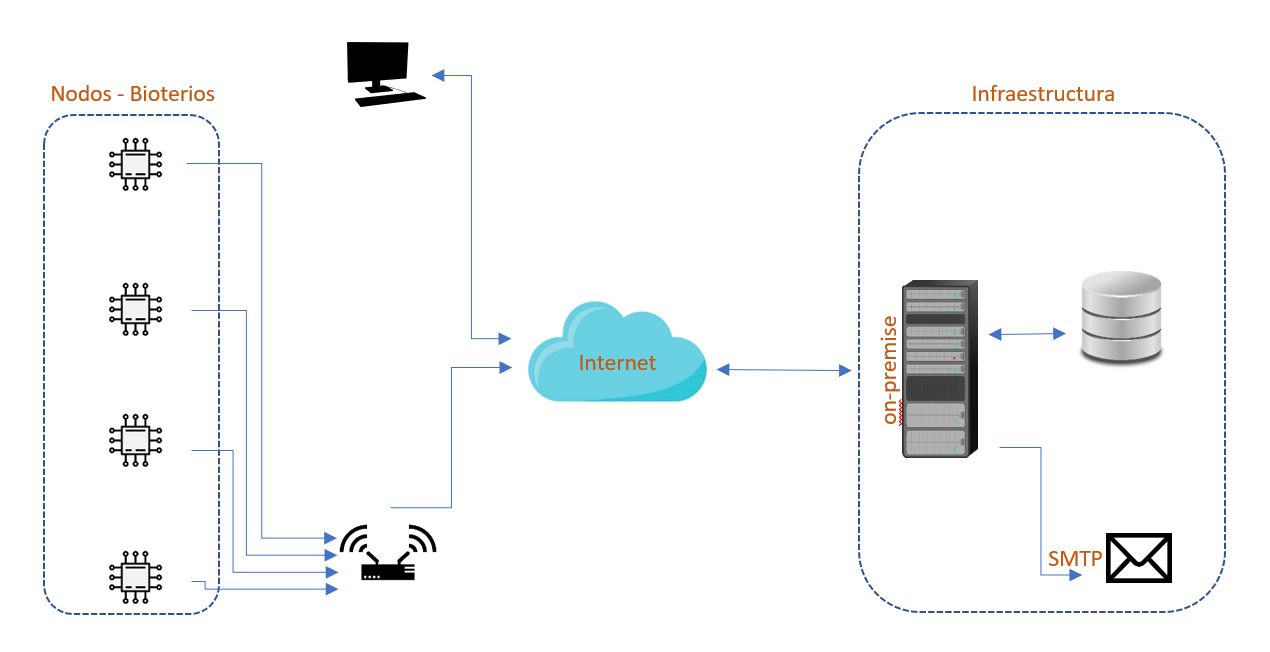
\includegraphics[width=.75\textwidth]{./Figuras/figura1.png}
%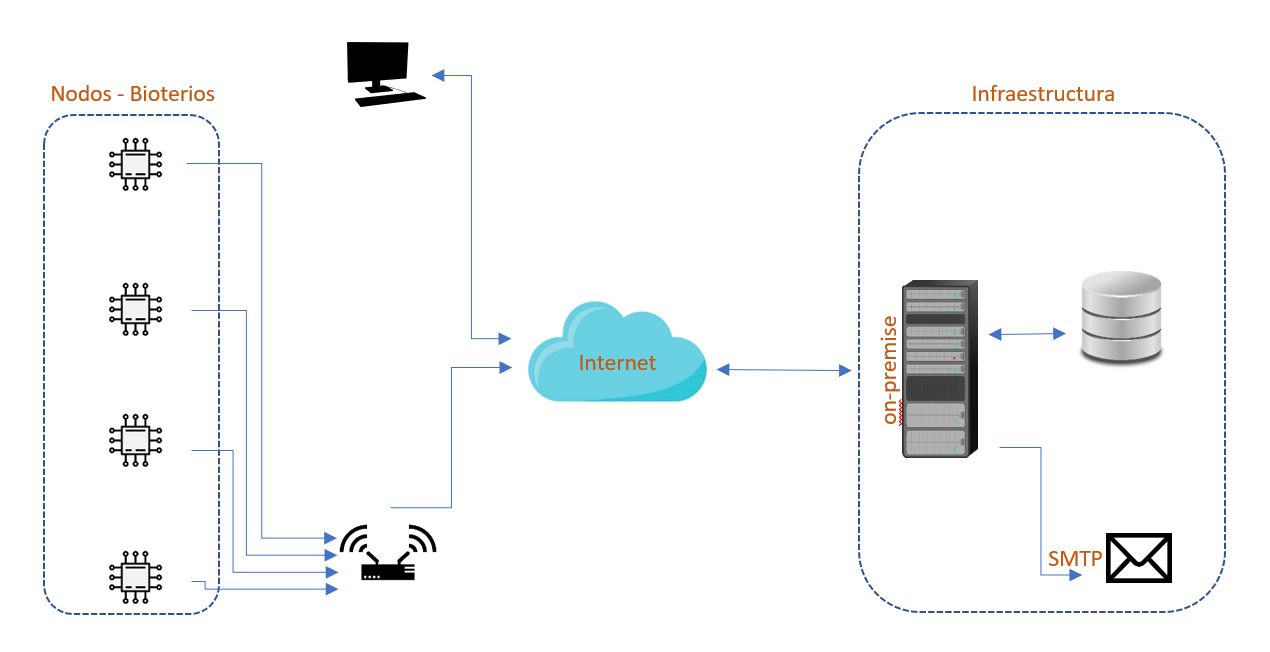
\includegraphics[width=.5\textwidth]{./Figuras/figura1.png}
\caption{Diagrama general del sistema.}
\label{fig:diagBloques}
\end{figure}

\vspace{25px}

\section{2. Identificación y análisis de los interesados}
\label{sec:interesados}

\begin{table}[ht]
%\caption{Identificación de los interesados}
%\label{tab:interesados}
\begin{tabularx}{\linewidth}{@{}|l|X|X|l|@{}}
\hline
\rowcolor[HTML]{C0C0C0} 
Rol           & Nombre y Apellido & Organización 	& Puesto 	\\ \hline
Cliente       & \clientename      &\empclientename	& Investigador \\ \hline
Responsable   & \authorname       & FIUBA        	& Alumno 	\\ \hline
Orientador    & \supname	      & \pertesupname 	& Director Trabajo final \\ \hline
\end{tabularx}
\end{table}

\begin{itemize}
	\item Cliente: Juan Rosa es riguroso y exigente en los detalles.
	\item Responsable: Norberto Rodríguez, único personal en el equipo de desarrollo.
\end{itemize}


\section{3. Propósito del proyecto}
\label{sec:proposito}
El propósito de este proyecto es desarrollar un dispositivo para el monitoreo de las condiciones ambientales del bioterio, que incluya el registro de la telemetría, sistematización u organización de los datos recolectados, presentación de alertas vía SMTP a los investigadores y análisis de información por medio de un tablero de mandos.

\section{4. Alcance del proyecto}
\label{sec:alcance}

El proyecto incluye el diseño, desarrollo e implementación del sistema en conjunto con un prototipo de dispositivo instalado en el bioterio.

Se desarrollarán las siguientes actividades:
\begin{itemize}
	\item Confección de un prototipo de dispositivo encargado de la telemetría.
	\item Configuración del servidor Ubuntu server GNU/Linux distribución basada en Debian.
	\item Instalación de la aplicación web.
	\item Instalación y configuración de la base de datos.
	\item Confección de un dashboard.
	\item Confección del módulo de alertas vía SMTP.
\end{itemize}


El presente proyecto no incluye:
\begin{itemize}
	\item Provisión de la infraestructura de datos e Internet.
	\item Certificaciones ante autoridades competentes.
	\item Desarrollos para la automatización del bioterio.
\end{itemize}

\section{5. Supuestos del proyecto}
\label{sec:supuestos}

Para el desarrollo del presente proyecto se supone que:
\begin{itemize}
	\item Los bioterios tendrán acceso a Internet.
	\item Se contará con los recursos humanos necesarios por parte del Instituto de Medicina Regional para llevar a cabo el proyecto.
	\item El Instituto de Medicina Regional brindará acceso a los servidores para la instalación y configuración de la aplicación.
	\item Para la puesta en producción se utilizará el servidor de correo electrónico del instituto.
	\item Existe la disponibilidad de los componentes necesarios para el desarrollo del prototipo.
\end{itemize}

\section{6. Requerimientos}
\label{sec:requerimientos}

Los requerimientos identificados son:
\begin{enumerate}
	\item Requerimientos de hardware de los nodos
		\begin{enumerate}
			\item Cada nodo debe estar conformado por un microcontrolador.
			\item El nodo debe ser capaz de medir la temperatura y humedad.
			\item El nodo debe ser capaz de medir la Luz que reciben los artrópodos.
			\item El nodo debe ser capaz de medir CO2 en el bioterio.
			\item Fuente de alimentación debe estar incluida.
			\item El nodo debe poseer un Módulo Wi-Fi para la comunicación.
		\end{enumerate}
	\item Requerimientos de software
		\begin{enumerate}
			\item El sistema debe permitir configurar los parámetros para las alertas.
			\item El usuario debe poder seleccionar el nodo a visualizar en el tablero de mandos.
			\item El sistema debe permitir asignar un nodo a un bioterio en particular.
		\end{enumerate}
	\item Requerimientos de presentación
		\begin{enumerate}
			\item El sistema debe proveer un tablero de mandos.
			\item El usuario debe poder visualizar la historia de la telemetría para un posterior análisis cuando se evalúe el desempeño de la colonia.
		\end{enumerate}
	\item Requerimientos de alertas
		\begin{enumerate}
			\item El sistema debe notificar al investigador sobre cambios en la telemetría mediante el envío de un correo electrónico.
			\item El usuario debe poder observar alertas en el tablero de mandos.
		\end{enumerate}
	\item Requerimientos de almacenamiento en la base de datos
		\begin{enumerate}
			\item Se debe almacenar la lectura de temperatura.
			\item Se debe almacenar la lectura de humedad.
			\item Se debe almacenar la lectura de cantidad de luz.
			\item Se debe almacenar la lectura de CO2.
			\item Se debe almacenar la lectura de fecha y hora de la telemetría.
		\end{enumerate}
\end{enumerate}

\section{7. Historias de usuarios (\textit{Product backlog})}
\label{sec:backlog}

Como criterio de ponderación se utilizó la serie de Fibonacci.

\begin{enumerate}
	\item Dificultad
		\begin{enumerate}
			\item Baja - peso 1.
			\item Media - peso 3.
			\item Alta - peso 5.
		\end{enumerate}
	\item Complejidad
		\begin{enumerate}
			\item Baja - peso 1.
			\item Media - peso 5.
			\item Alta - peso 13.
		\end{enumerate}
	\item Riesgo o incertidumbre
		\begin{enumerate}
			\item Bajo - peso 2.
			\item Medio - peso 3.
			\item Alto - peso 5.
		\end{enumerate}
\end{enumerate}

\begin{itemize}
	\item Como investigador deseo poder visualizar la temperatura del bioterio para que el cambio de temperatura no comprometa la colonia de artrópodos y tomar acciones preventivas, por ejemplo el corte de energía eléctrica que afectan a los aires acondicionados.		
	Ponderación: 13.
	
	Dificultad: media (3).
	
	Complejidad: media (5).
	
	Riesgo: medio (3).
	
	(3 + 5 + 3 = 11 valor siguiente de la serie Fibonacci 13).

	\item Como investigador deseo poder visualizar la humedad del bioterio para que no se vea comprometida la colonia de artrópodos.
	Ponderación: 13.
	
	Dificultad: media (3).
	
	Complejidad: media (5).
	
	Riesgo: medio (3).
	
	(3 + 5 + 3 = 11 valor siguiente de la serie Fibonacci 13).
	
	\item Como investigador deseo poder visualizar la cantidad de luz recibida para  que no afecte a la colonia de artrópodos a largo plazo.
	Ponderación: 21.
	
	Dificultad: alta (5).
	
	Complejidad: medio (5).
	
	Riesgo: medio (3).
	
	(5 + 5 + 3 = 13 valor siguiente de la serie Fibonacci 21).
	
	\item Como investigador deseo poder visualizar la cantidad de CO2 del bioterio para que no se vea comprometida la colonia de artrópodos.
	Ponderación: 13.
	
	Dificultad: baja (1).
	
	Complejidad: media (5).
	
	Riesgo: bajo (2).
	
	(1 + 5 + 2 = 8 valor siguiente de la serie Fibonacci 13).
	
	\item Como investigador deseo poder consultar los datos registrados con anterioridad para medir o comparar su impacto en la evolución de la colonia.
	Ponderación: 34.
	
	Dificultad: alta (5).
	
	Complejidad: alta (13).
	
	Riesgo: medio (3).
	
	(5 + 13 + 3 = 21 valor siguiente de la serie Fibonacci 34).
	
	\item Como investigador deseo recibir alertas por correo electrónico ante cambios en las condiciones del bioterio y así poder tomar medidas correctivas.
	Ponderación: 34.
	
	Dificultad: alta (5).
	
	Complejidad: alta (13).
	
	Riesgo: alto (5).
	
	(5 + 13 + 5 = 23 valor siguiente de la serie Fibonacci 34).
	
	\item Como investigador deseo poder visualizar un tablero de mandos independientemente de mi ubicación para supervisar el bioterio.
	Ponderación: 34.
	
	Dificultad: media (3).
	
	Complejidad: alta (13).
	
	Riesgo: alto (5).
	
	(3 + 13 + 5 = 21 valor siguiente de la serie Fibonacci 34).
	
\end{itemize}

\section{8. Se incluyen los siguietes entregables:}
\label{sec:entregables}

\begin{itemize}
	\item Manual de uso.
	\item Diagrama del sistema.
	\item Código fuente del firmware.
	\item Código fuente del la aplicación.
	\item Un prototipo de nodo.
	\item Informe de avance.
	\item Memoria escrita.
\end{itemize}

\section{9. Desglose del trabajo en tareas}
\label{sec:wbs}

\begin{enumerate}
\item Investigación y planificación del proyecto. (60 hs)
	\begin{enumerate}
	\item Seleccionar la arquitectura para el sistema. (5 hs)
	\item Investigar tecnologías IoT. (15 hs)
	\item Investigar sensores. (15 hs)
	\item Investigar microcontroladores. (15 hs)
	\item Investigar arquitecturas de microservicios. (10 hs)
	\end{enumerate}
\item Adquisición de componentes. (10 hs)
	\begin{enumerate}
	\item Consultar costos de los componentes. (5 hs)
	\item Realizar los pedidos a proveedores. (5 hs)
	\end{enumerate}
\item Instalación e implementación de la base de datos. (20 hs)
	\begin{enumerate}
	\item Instalación. (8 hs)
	\item Creación y configuración (12 hs)

	\end{enumerate}
\item Desarrollo del sistema - back-end. (120 hs)
	\begin{enumerate}
	\item Instalación de entorno de trabajo. (40 hs)
	\item Desarrollo de API. (40 hs)
	\item Desarrollo de alertas. (40 hs)
	\end{enumerate}
\item Desarrollo del sistema - front-end. (120 hs)
	\begin{enumerate}
	\item Desarrollo de acceso al sistema. (20 hs)
	\item Desarrollo del tablero de mandos. (45 hs)
	\item Desarrollo de visualización histórica de telemetría. (15 hs)
	\item Desarrollo de configuración de alertas. (25 hs)
	\item Desarrollo del menú de opciones. (5 hs)
	\item Desarrollo de ajustes de dispositivos. (5 hs)
	\item Desarrollo de ajustes de usuarios. (5 hs)
	\end{enumerate}
\item Desarrollo de firmware - módulo de temperatura y humedad. (85 hs)
	\begin{enumerate}
	\item Construcción del módulo e integración de componentes. (20 hs)
	\item Desarrollo del firmware para lectura de datos. (40 hs)
	\item Prueba de conexión con la aplicación. (25 hs)
	\end{enumerate}
\item Desarrollo de firmware - módulo de luz. (55 hs)
	\begin{enumerate}
	\item Construcción del módulo e integración de componentes. (10 hs)
	\item Desarrollo del Firmware para lectura de datos. (30 hs)
	\item Prueba de conexión con la aplicación. (15 hs)
	\end{enumerate}
\item Desarrollo de firmware - módulo de CO2. (55 hs)
	\begin{enumerate}
	\item Construcción del módulo e integración de componentes. (10 hs)
	\item Desarrollo del firmware para lectura de datos. (30 hs)
	\item Prueba de conexión con la aplicación. (15 hs)
	\end{enumerate}
\item Testing. (30 hs)
	\begin{enumerate}
	\item Prueba de conectividad. (2 hs)
	\item Prueba de sensores. (3 hs)
	\item Prueba del tablero de mandos. (4 hs)
	\item Prueba de alertas. (4 hs)
	\item Verificación y validación del sistema completo. (10 hs)
	\item Prueba del prototipo en ambiente real. (7 hs)
	\end{enumerate}
\item Presentación del proyecto y cierre. (45 hs)
	\begin{enumerate}
	\item Escritura del informe de avance. (15 hs)
	\item Escritura de la memoria escrita. (15 hs)
	\item Escritura del plan de trabajo final. (15 hs)
	\end{enumerate}
\end{enumerate}

Cantidad total de horas: (600 hs)

\section{10. Diagrama de activity on node}
\label{sec:AoN}

%\begin{consigna}{red}
%Armar el AoN a partir del WBS definido en la etapa anterior. 

%La figura \ref{fig:AoN} fue elaborada con el paquete latex tikz y pueden consultar la siguiente referencia \textit{online}:

%\url{https://www.overleaf.com/learn/latex/LaTeX_Graphics_using_TikZ:_A_Tutorial_for_Beginners_(Part_3)\%E2\%80\%94Creating_Flowcharts}

%\end{consigna}

\begin{figure}[htpb]
\centering 
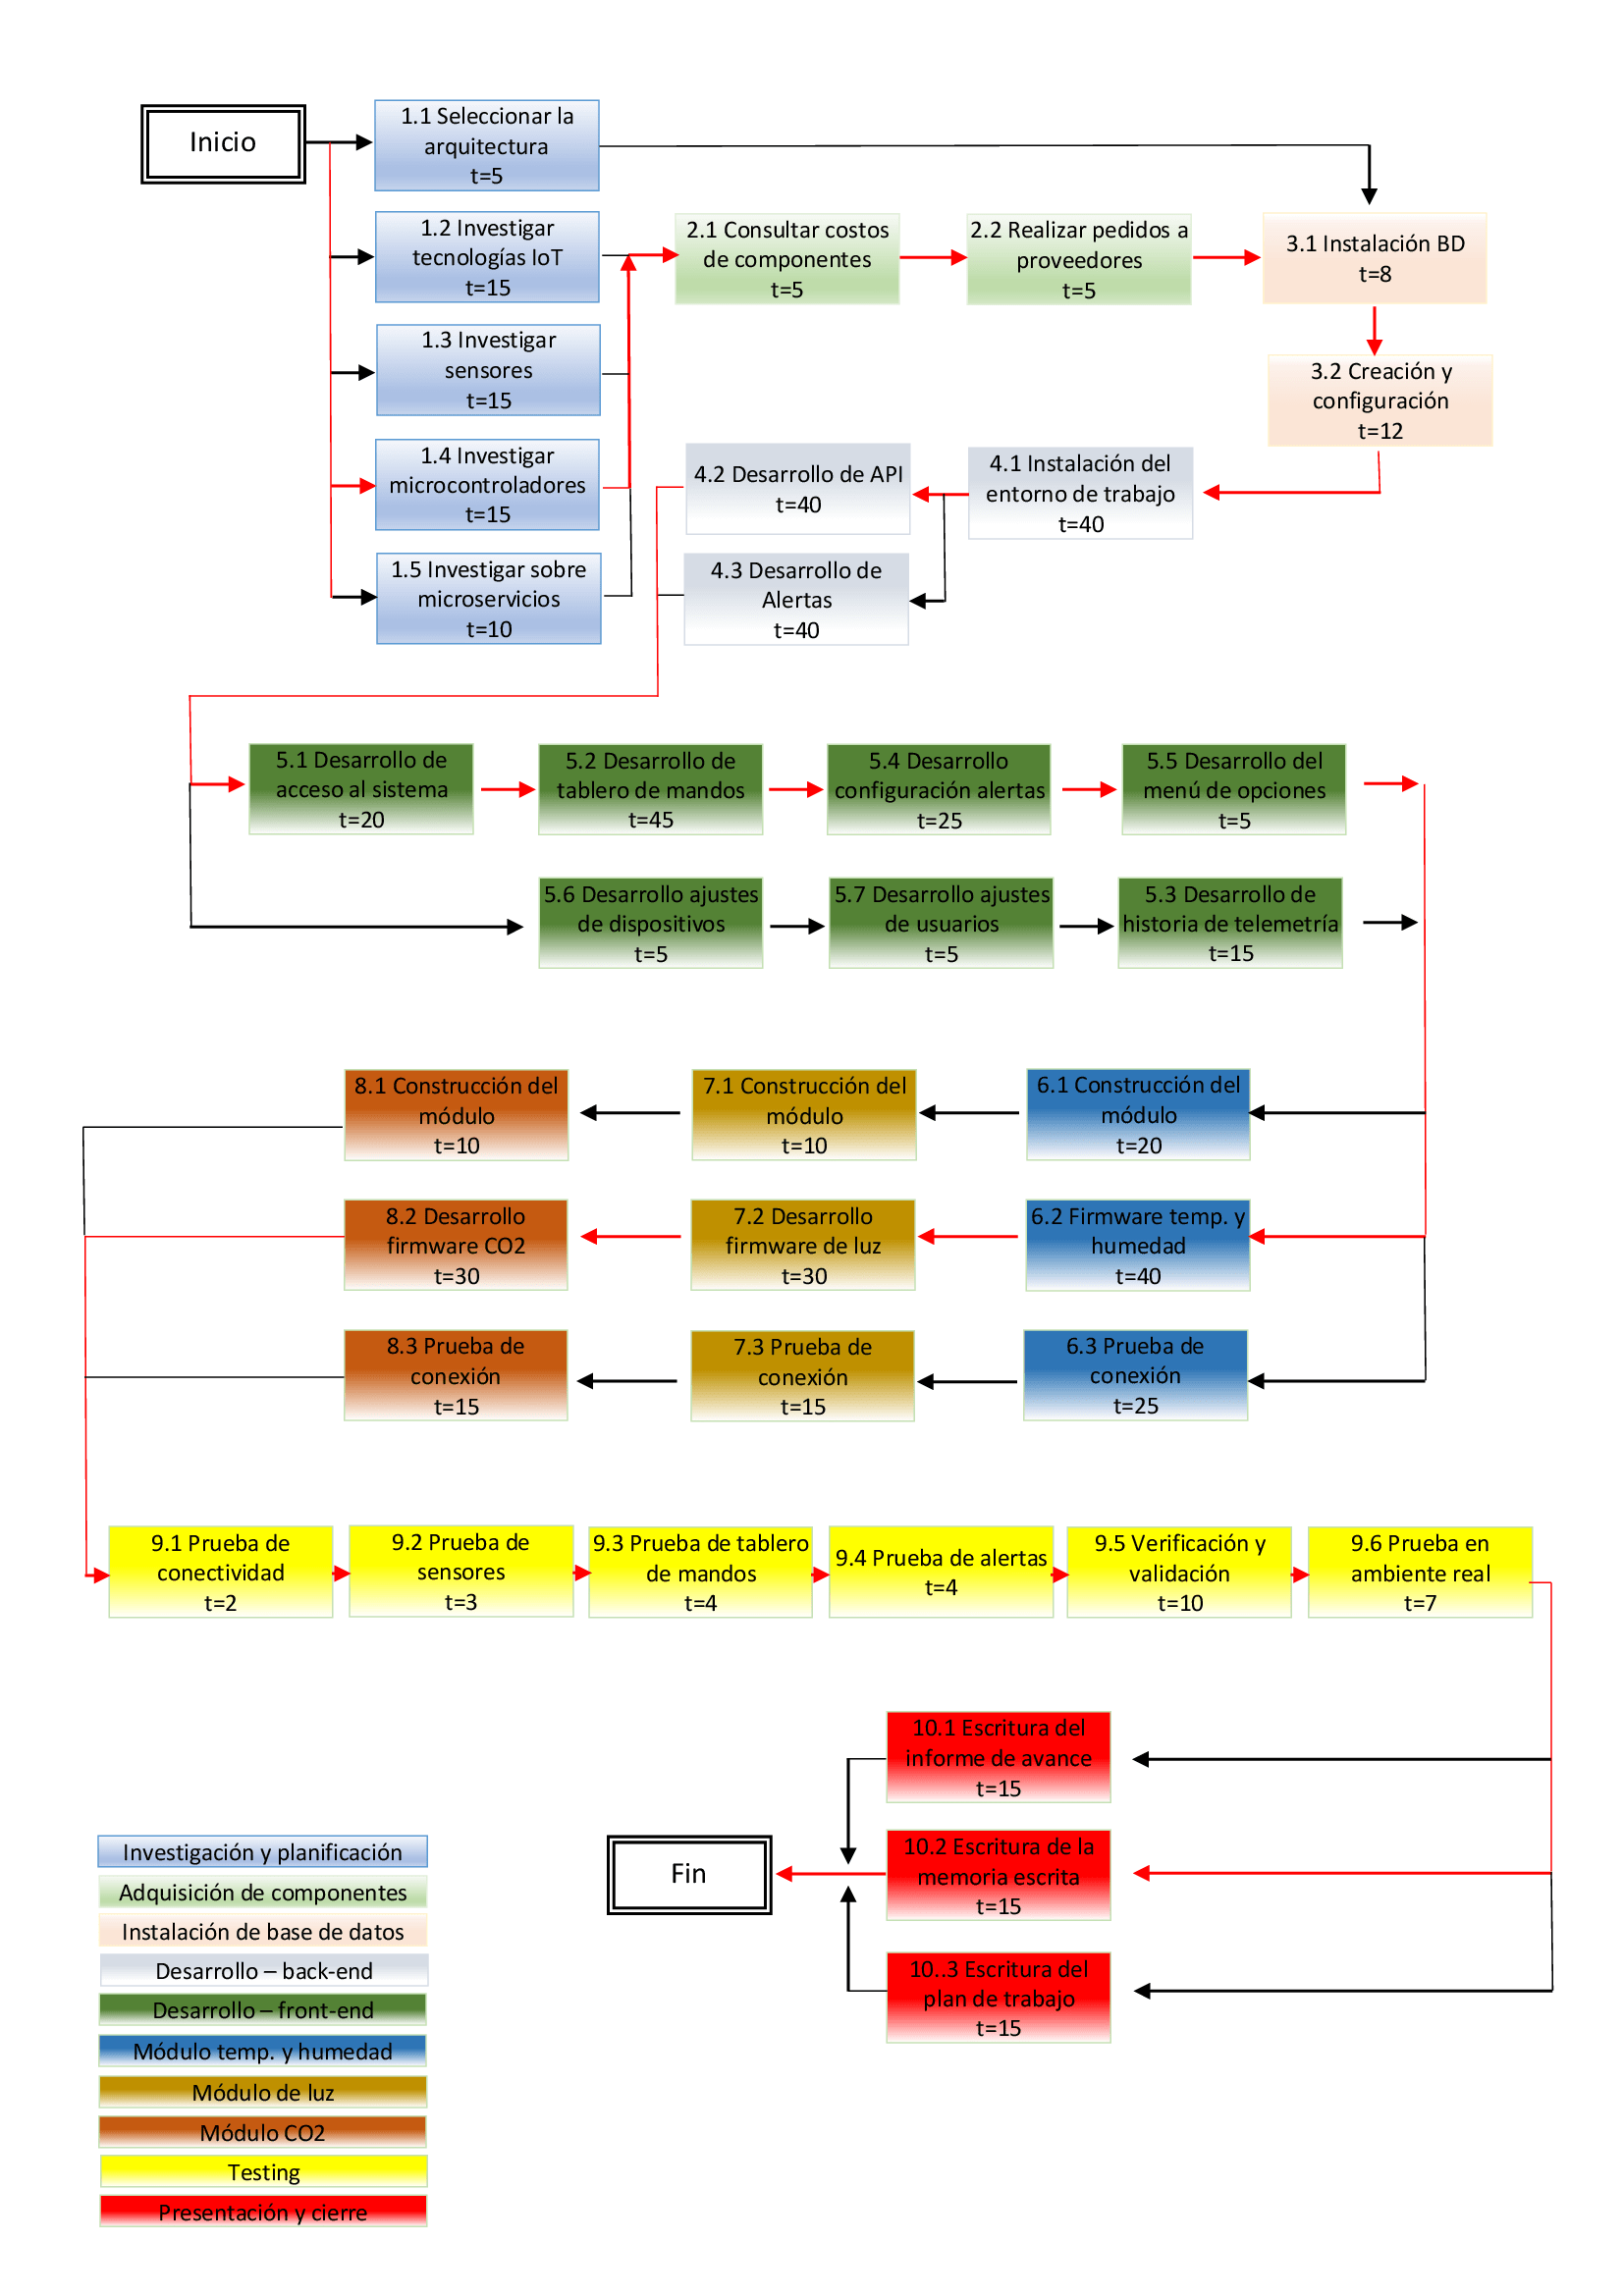
\includegraphics[height=1.49\textwidth]{./Figuras/AoN.png}
%\includegraphics[height=1.5\textwidth]{./Figuras/ActivityOnNode.png}
%\includegraphics[height=.85\textheight]{./Figuras/Gantt-2.png}
\caption{Diagrama en \textit{activity on node}.}
\label{fig:AoN}
\end{figure}

En la figura 2 se muestra el diagrama activity on node, la unidad de tiempo está expresada en horas. Las líneas en color rojo indica el camino crítico.



\section{11. Diagrama de Gantt}
\label{sec:gantt}

\begin{figure}[htpb]
\centering 
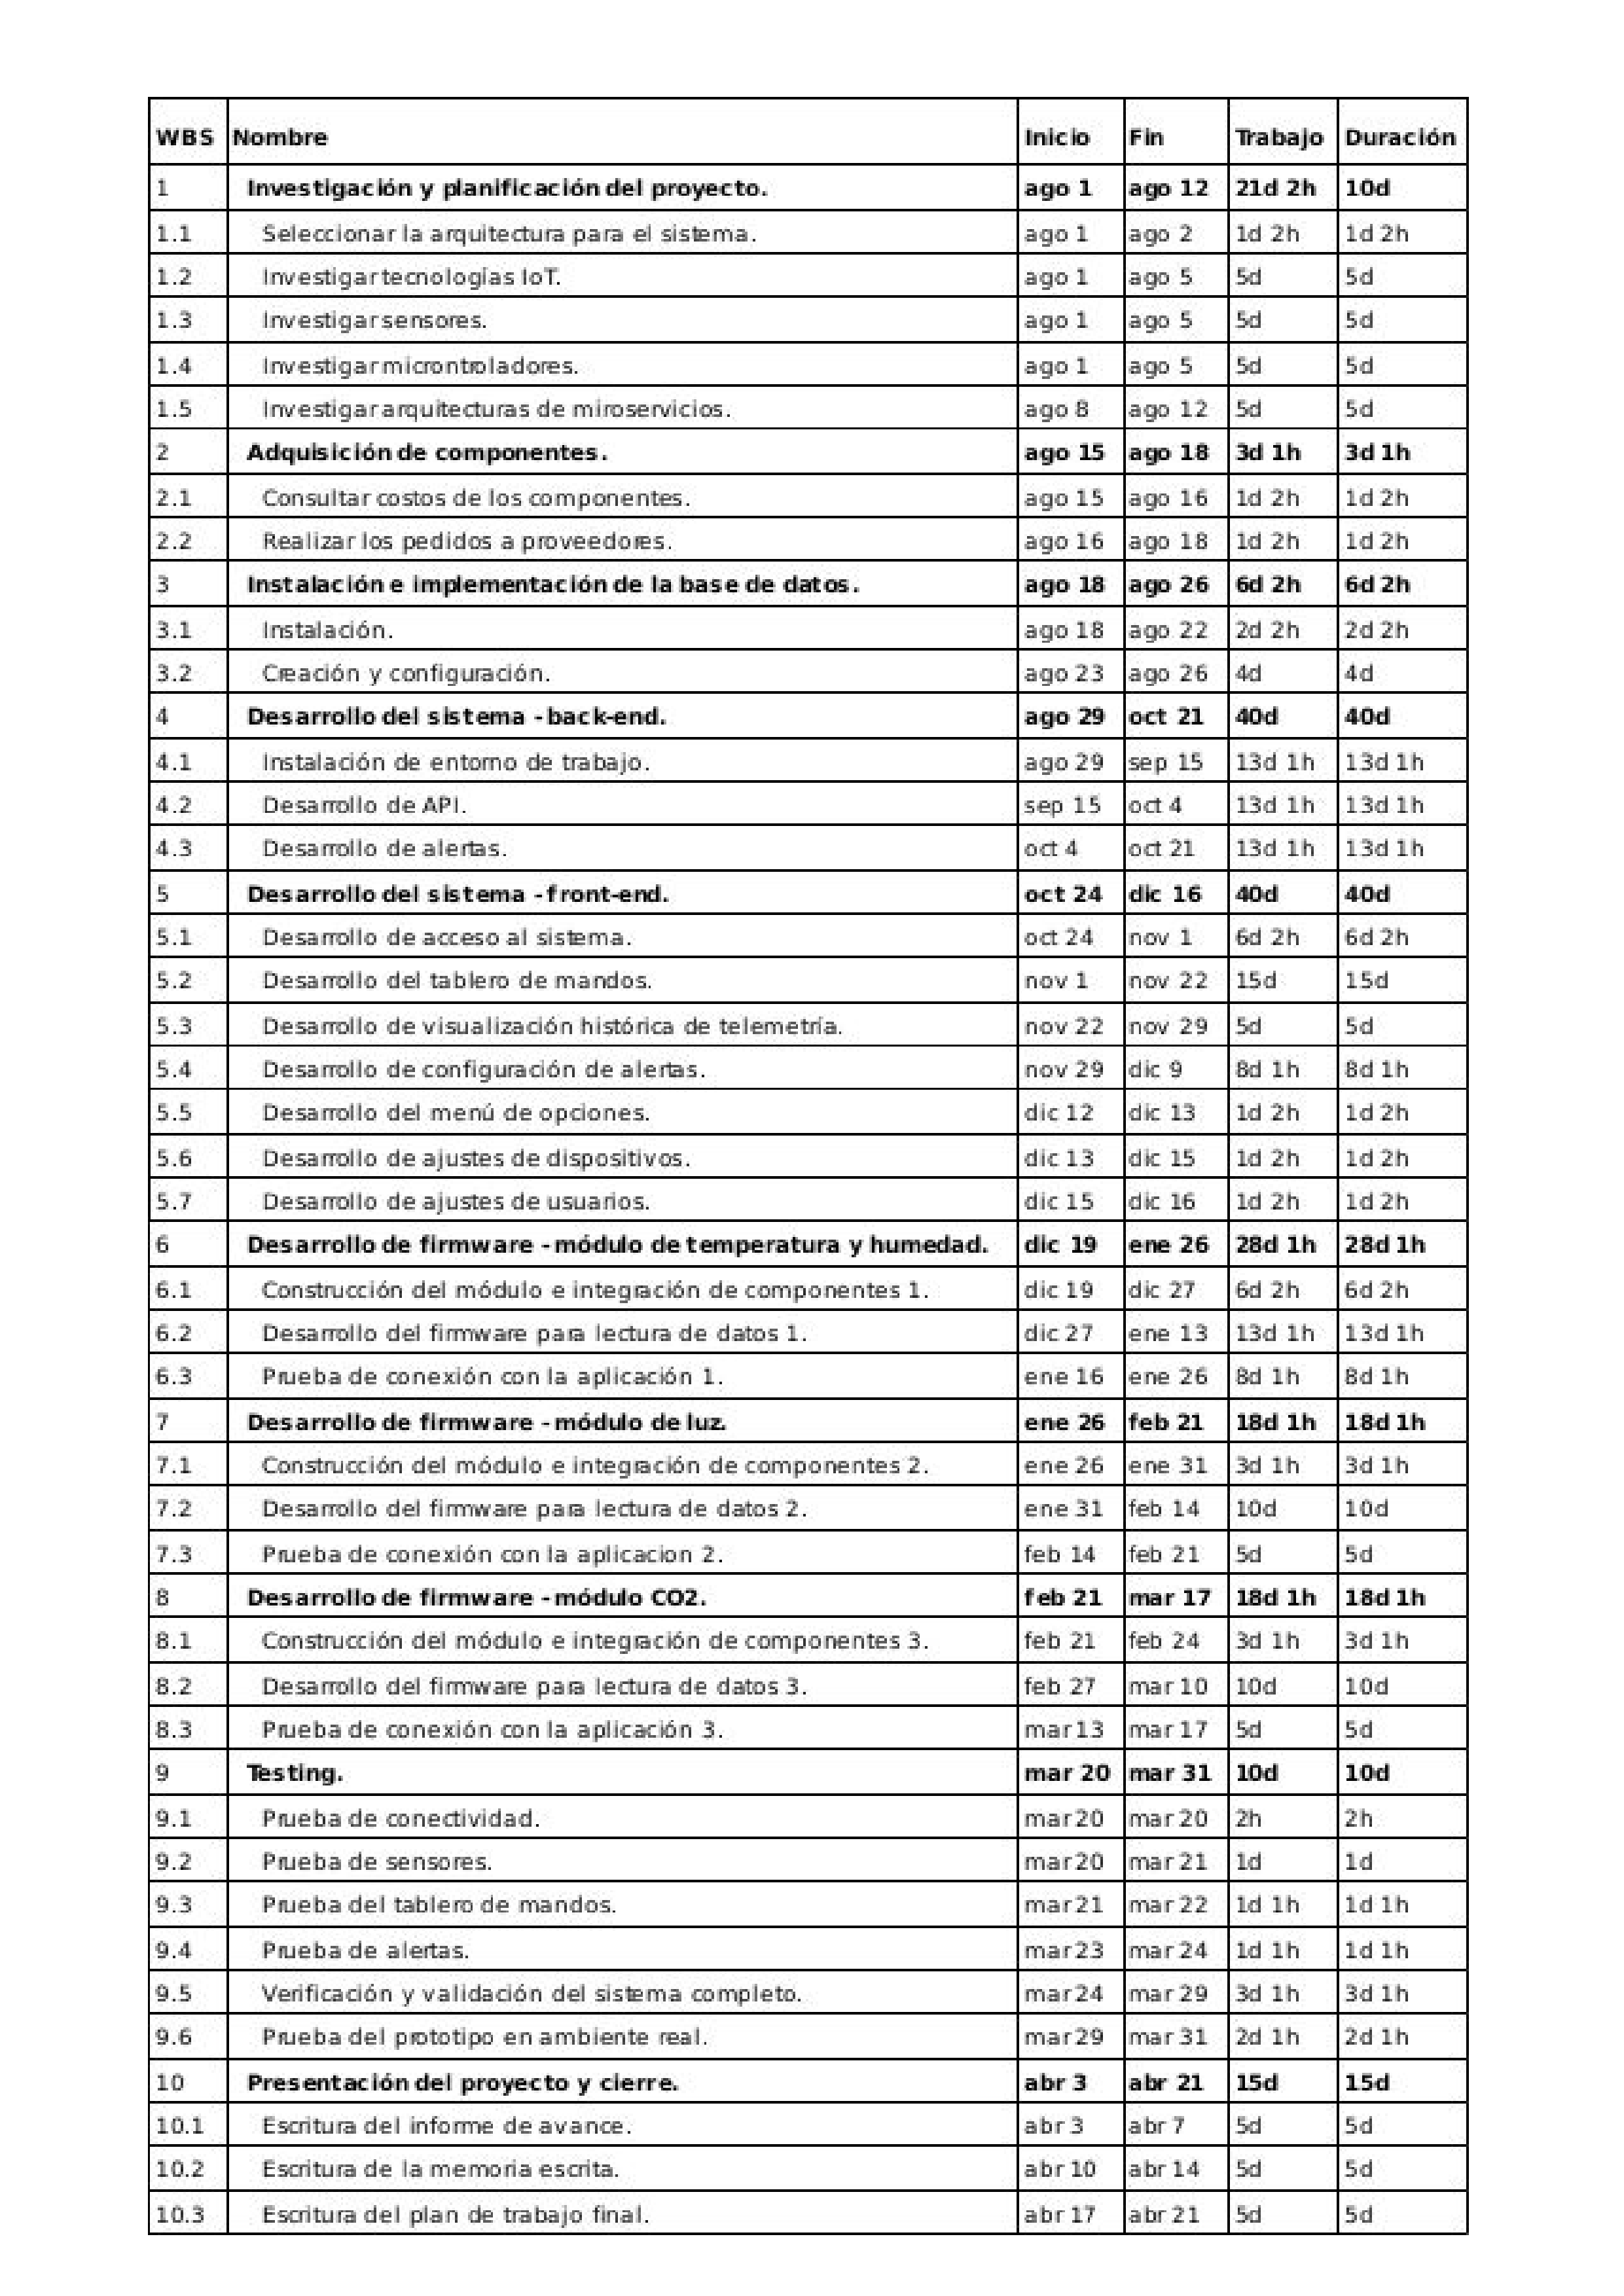
\includegraphics[width=.50\textheight]{./Figuras/Tareas.png}
\caption{Tabla de actividades.}
\label{fig:AoN}
\end{figure}

%\begin{figure}[htbp]
%\begin{center}
%\begin{ganttchart}{1}{12}
%  \gantttitle{2020}{12} \\
%  \gantttitlelist{1,...,12}{1} \\
%  \ganttgroup{Investigación y planificación del proyecto.}{1}{2} \\
%  \ganttbar{Seleccionar la arquitectura para el sistema.}{1}{2} \\
%  \ganttlinkedbar{Investigar tecnologías IoT.}{3}{7} \ganttnewline
%  \ganttmilestone{Milestone o hito}{7} \ganttnewline
%  \ganttbar{Final Task}{8}{12}
%  \ganttlink{elem2}{elem3}
%  \ganttlink{elem3}{elem4}  
%  \ganttgroup{Adquisición de componentes.}{1}{7} \\
%  \ganttbar{Task 1}{1}{2} \\
%  \ganttlinkedbar{Task 2}{3}{7} \ganttnewline
%  \ganttmilestone{Milestone o hito}{7} \ganttnewline
%  \ganttbar{Final Task}{8}{12}
%  \ganttlink{elem2}{elem3}
%  \ganttlink{elem3}{elem4}
%\end{ganttchart}
%\end{center}
%\caption{Diagrama de gantt de ejemplo}
%\label{fig:gantt}
%\end{figure}

%\begin{consigna}{red}
%Existen muchos programas y recursos \textit{online} para hacer diagramas de gantt, %entre los cuales destacamos:
En la figura 3 se puede ver la tabla de actividades. En las figuras 4 y 5 se observa el diagrama de Gantt. Se calcula una jornada diaria de trabajo de 8hs.

%\begin{figure}[htbp]
%\begin{center}
%\begin{ganttchart}{1}{12}
%  \gantttitle{2020}{12} \\
%  \gantttitlelist{1,...,12}{1} \\
%  \ganttgroup{Group 1}{1}{7} \\
%  \ganttbar{Task 1}{1}{2} \\
%  \ganttlinkedbar{Task 2}{3}{7} \ganttnewline
%  \ganttmilestone{Milestone o hito}{7} \ganttnewline
%  \ganttbar{Final Task}{8}{12}
%  \ganttlink{elem2}{elem3}
%  \ganttlink{elem3}{elem4}
%\end{ganttchart}
%\end{center}
%\caption{Diagrama de gantt de ejemplo}
%\label{fig:gantt}
%\end{figure}

\begin{landscape}
\begin{figure}[htpb]
\centering 
%\includegraphics[height=.85\textheight]{./Figuras/Gantt-2.png}
%\includegraphics[width=1\textheight]{./Figuras/Gantt1.png}
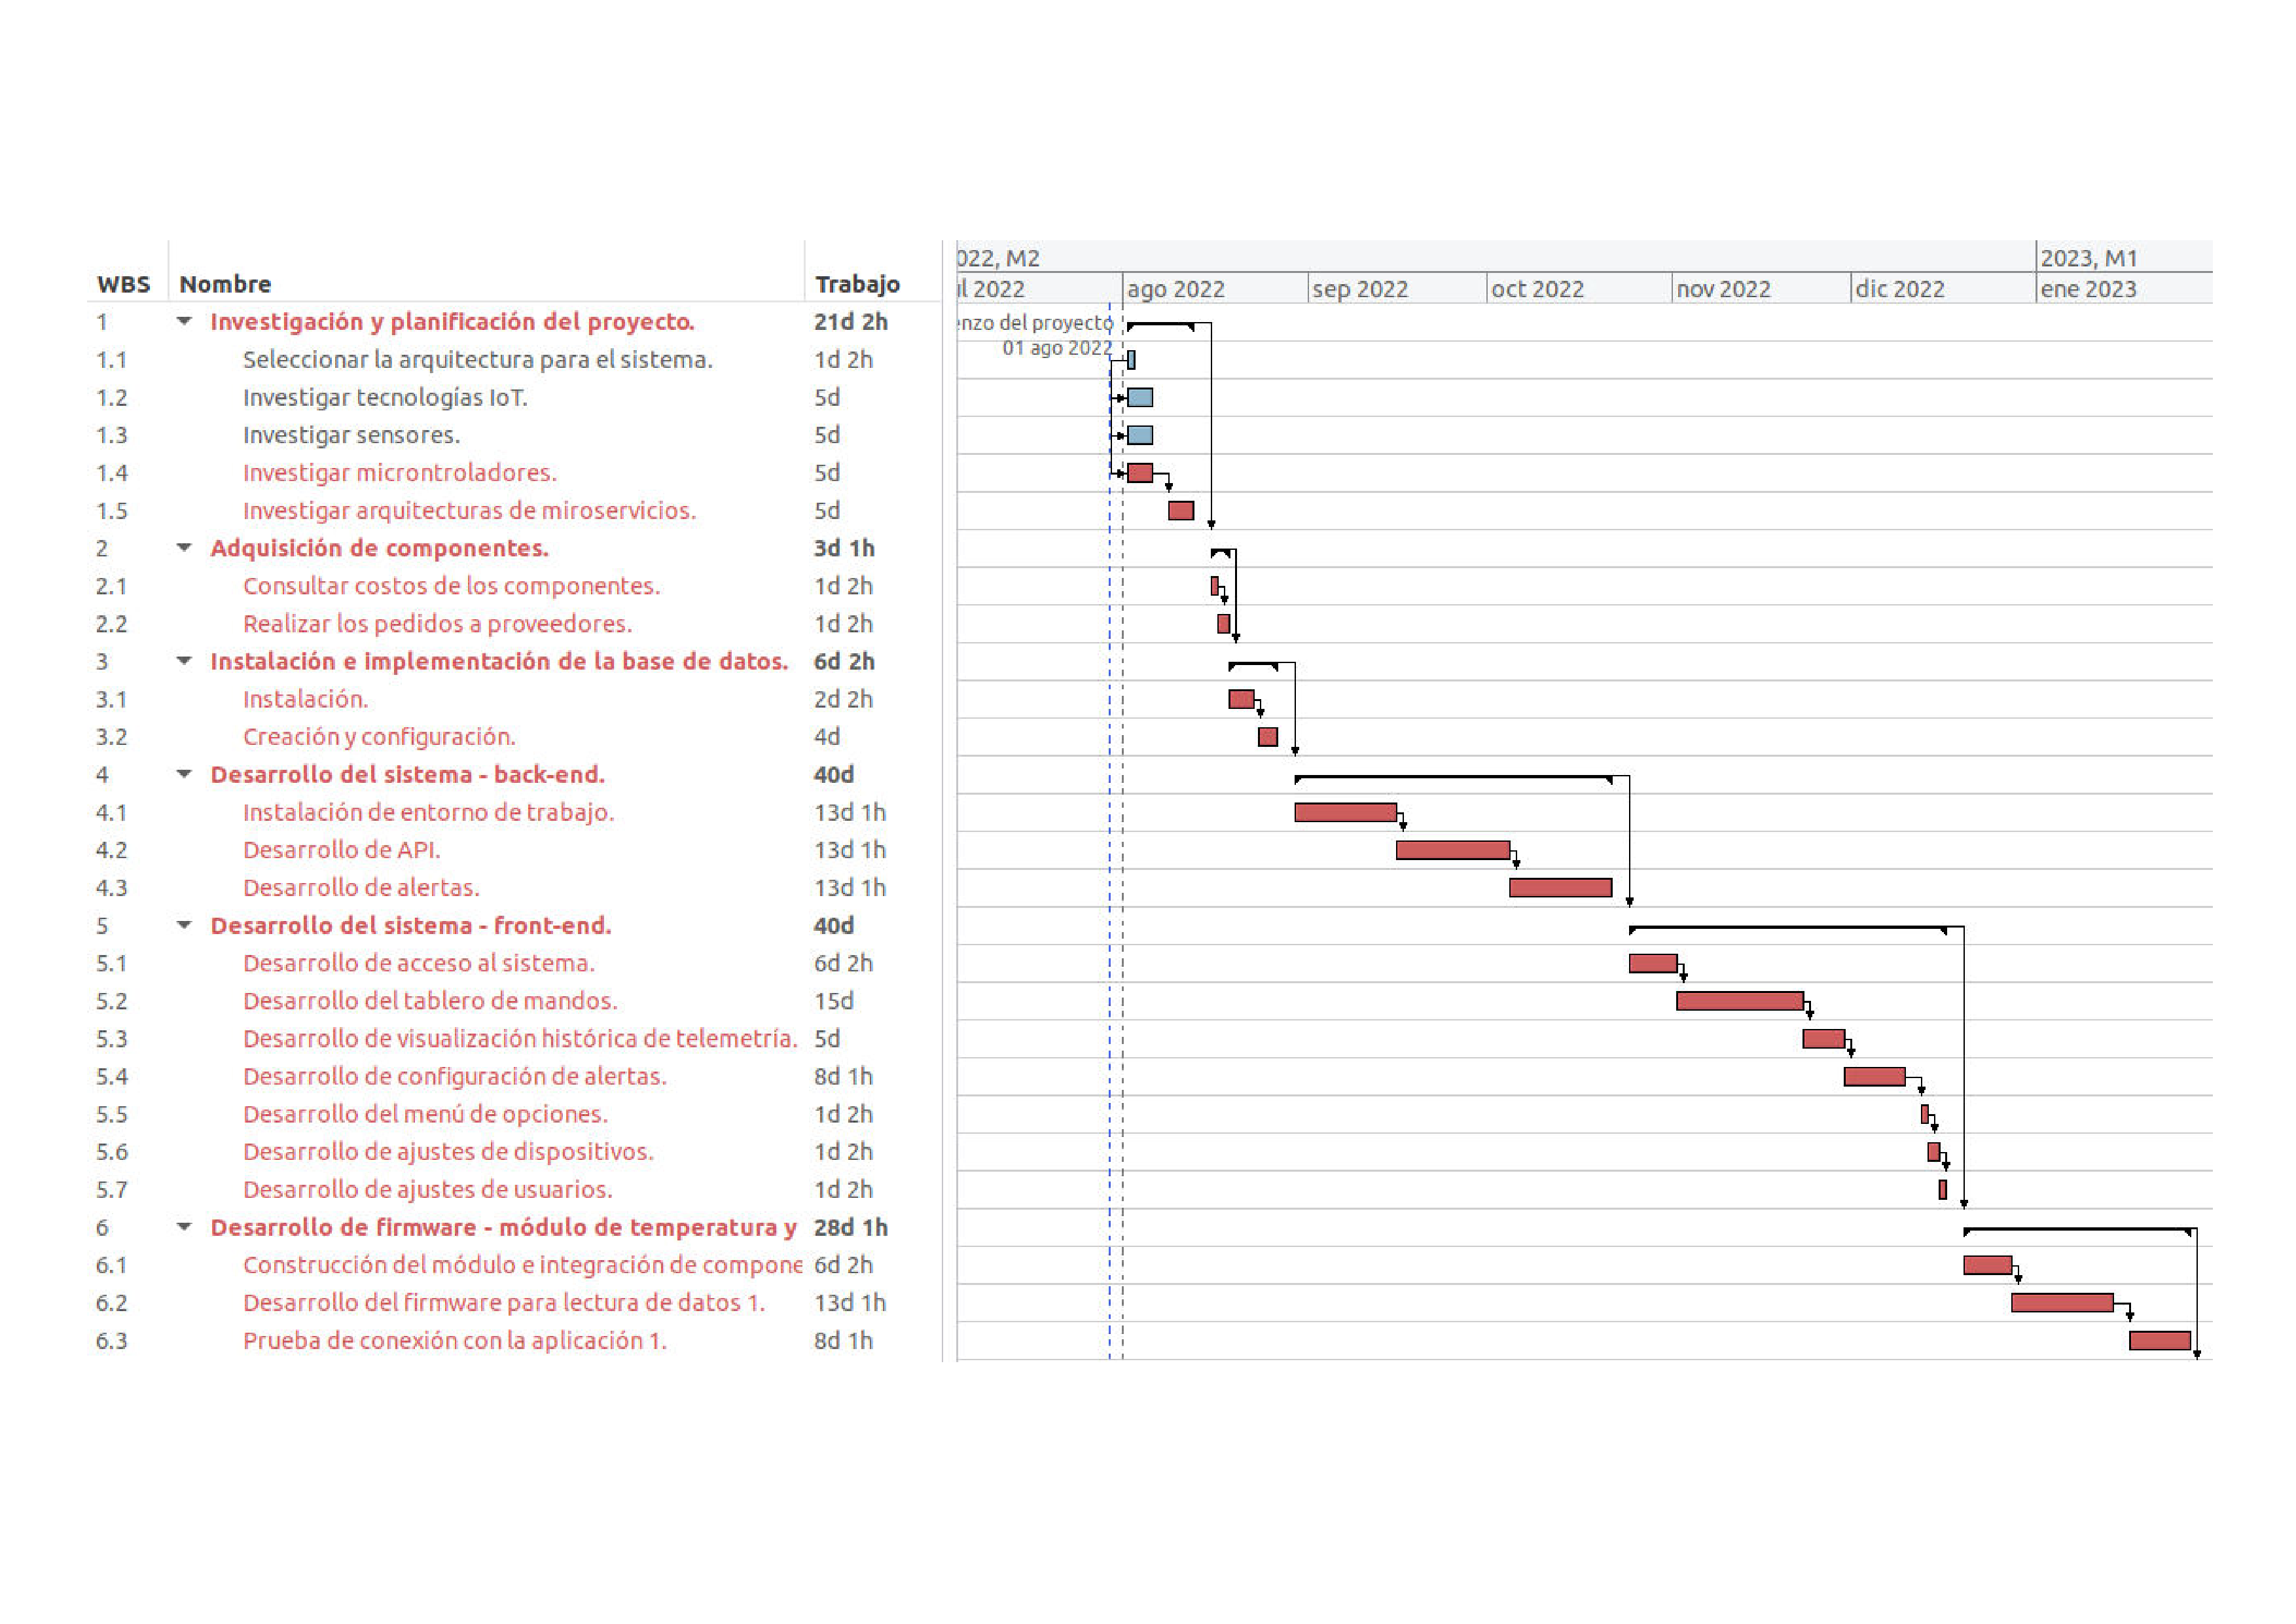
\includegraphics[height=.85\textheight]{./Figuras/DiagramaGantt_1.png}
\caption{Diagrama de Gantt parte 1/2.}
\label{fig:diagGantt}
\end{figure}
\end{landscape}
%\end{consigna}

\begin{landscape}
\begin{figure}[htpb]
\centering 
%\includegraphics[height=.85\textheight]{./Figuras/Gantt-2.png}
%\includegraphics[width=1\textheight]{./Figuras/Gantt1.png}
%\includegraphics[height=.57\textheight]{./Figuras/Gantt2.png}
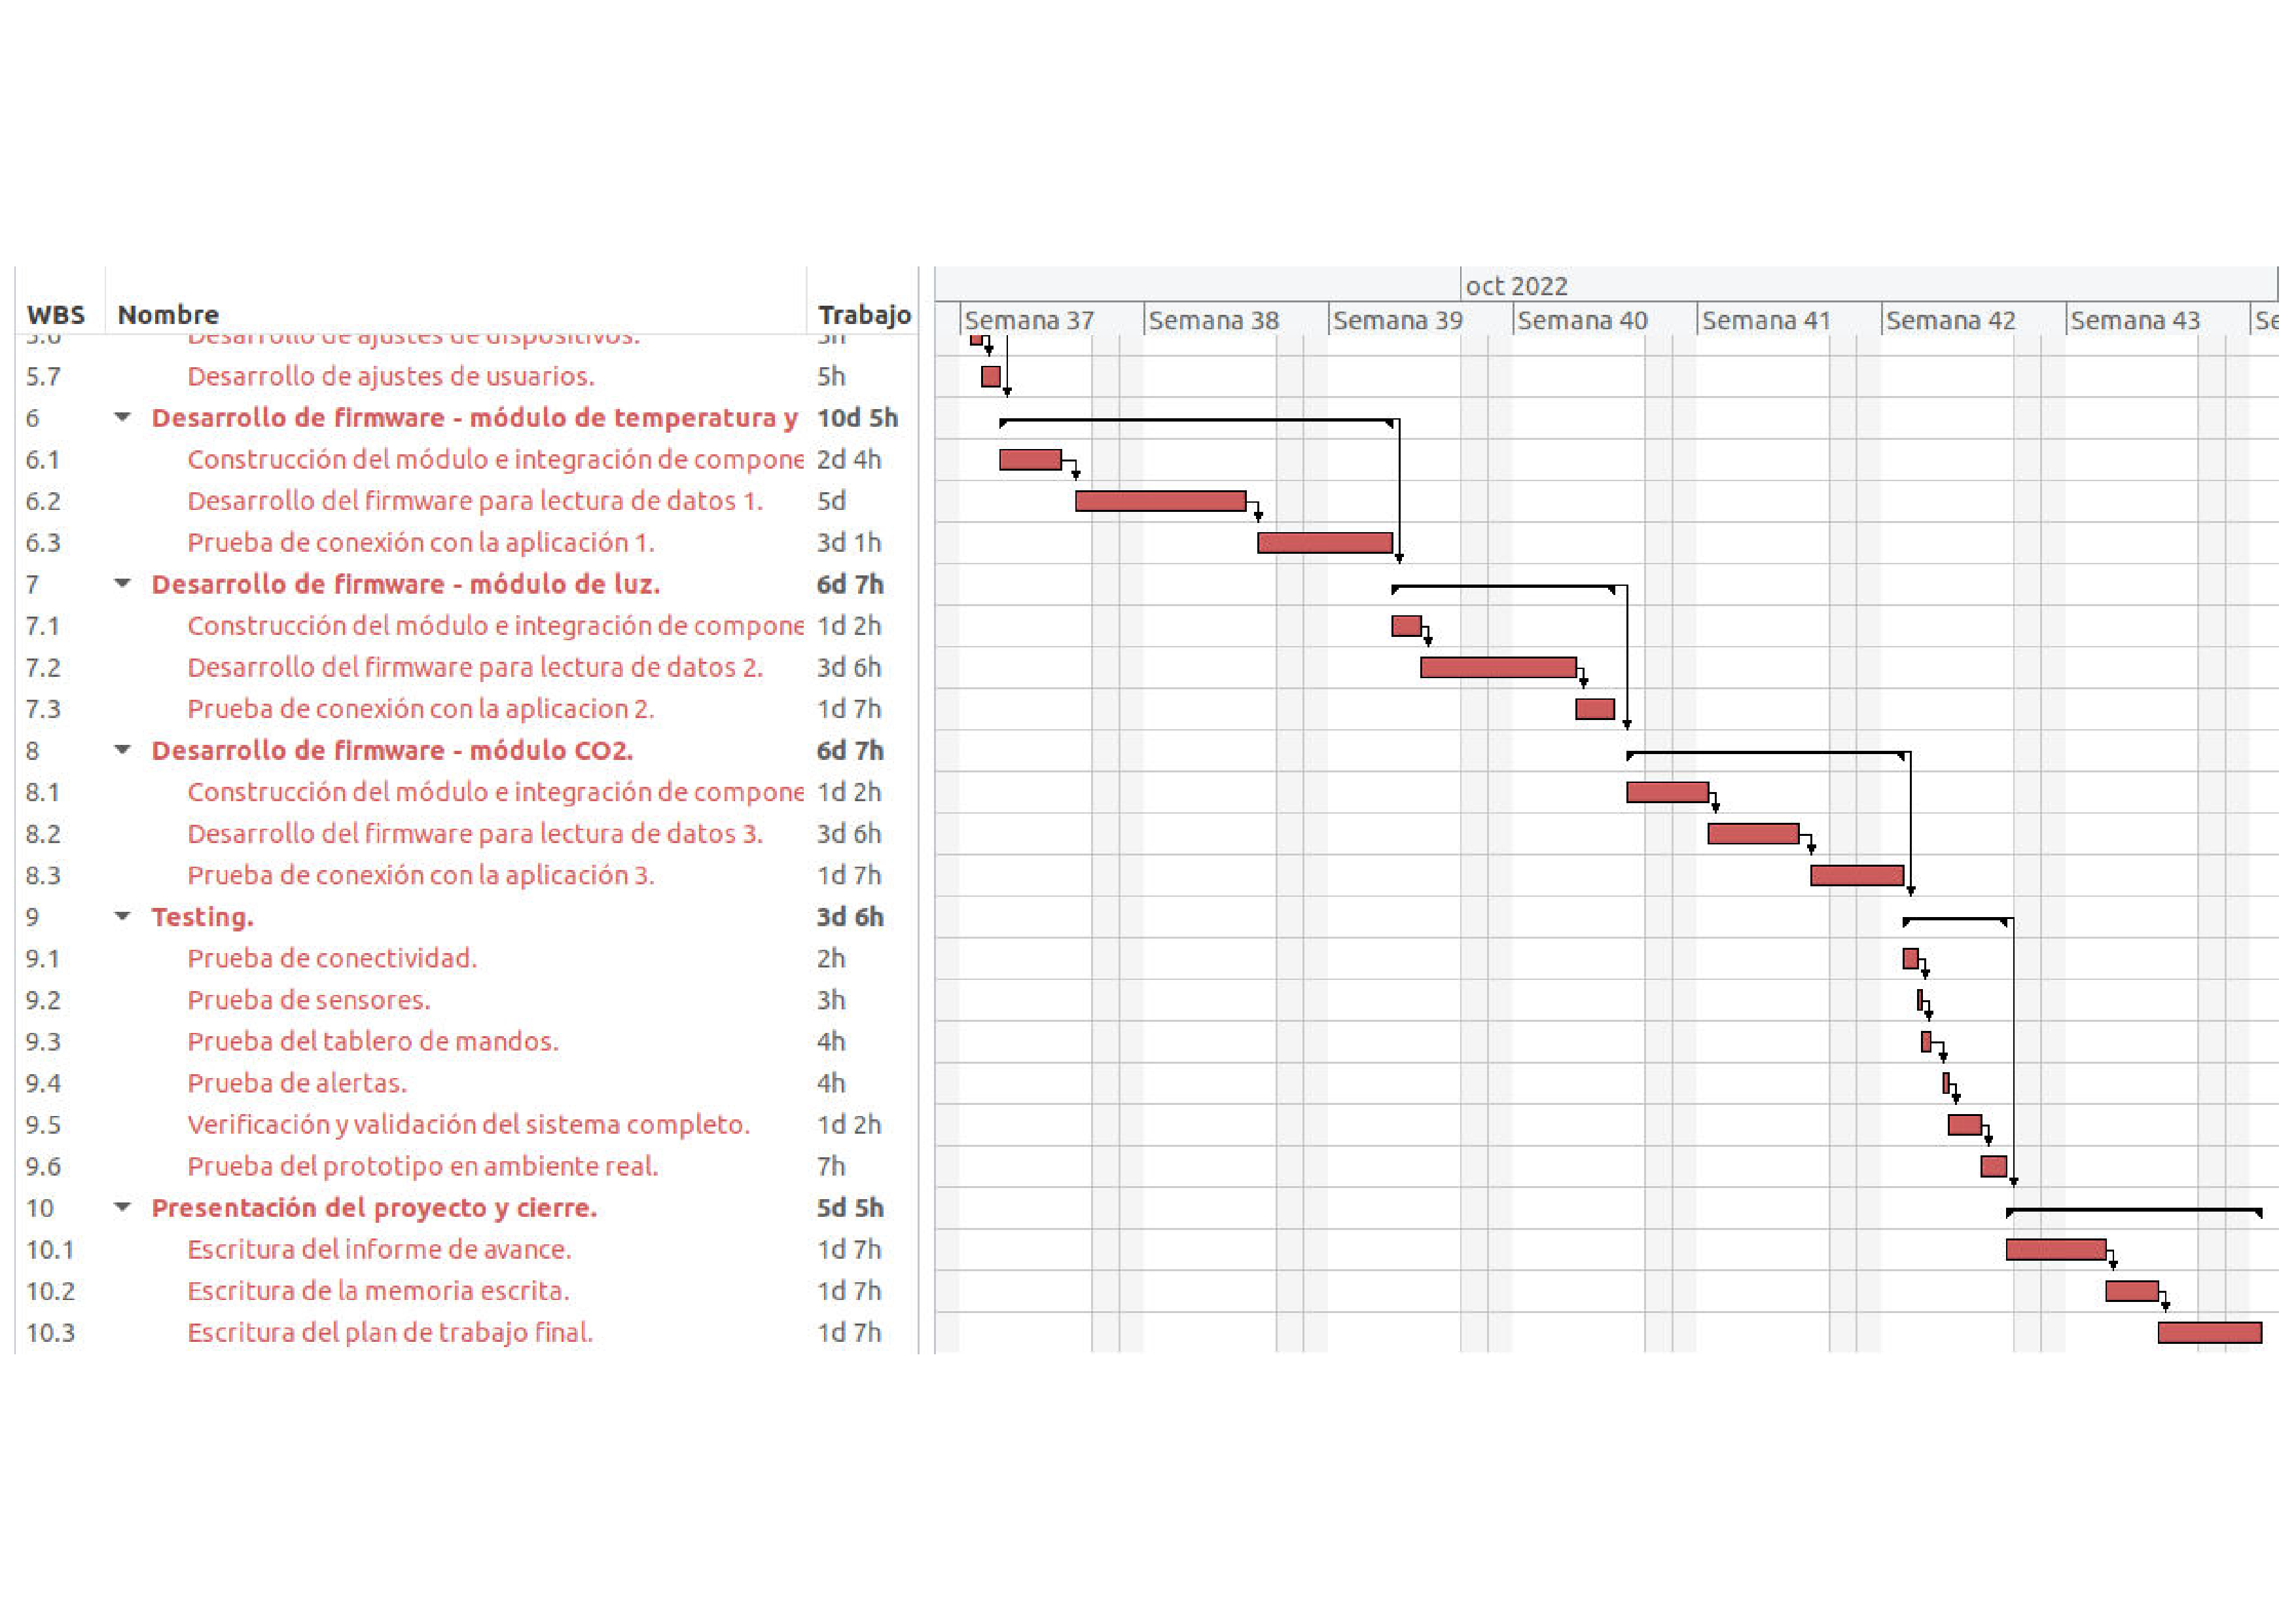
\includegraphics[height=.85\textheight]{./Figuras/DiagramaGantt_2.png}
\caption{Diagrama de Gantt parte 2/2.}
\label{fig:diagGantt}
\end{figure}
\end{landscape}



\section{12. Presupuesto detallado del proyecto}
\label{sec:presupuesto}

% Please add the following required packages to your document preamble:
% \usepackage[table,xcdraw]{xcolor}
% If you use beamer only pass "xcolor=table" option, i.e. \documentclass[xcolor=table]{beamer}
\begin{table}[htpb]
\centering
\begin{tabular}{|lccc|}
\hline
\rowcolor[HTML]{C0C0C0} 
\multicolumn{4}{|c|}{\cellcolor[HTML]{C0C0C0}{\color[HTML]{000000} COSTOS DIRECTOS}}                                                                                                                                                                                                      \\ \hline
\rowcolor[HTML]{C0C0C0} 
\multicolumn{1}{|c|}{\cellcolor[HTML]{C0C0C0}{\color[HTML]{000000} Descripción}} & \multicolumn{1}{c|}{\cellcolor[HTML]{C0C0C0}{\color[HTML]{000000} Cantidad}} & \multicolumn{1}{c|}{\cellcolor[HTML]{C0C0C0}{\color[HTML]{000000} Valor unitario}} & {\color[HTML]{000000} Valor Total} \\ \hline
\multicolumn{1}{|l|}{Horas de ingeniería}                                        & \multicolumn{1}{c|}{600}                                                     & \multicolumn{1}{c|}{1560,00}                                                        & 936.000,00                         \\ \hline
\multicolumn{1}{|l|}{Placa esp-wroom-32}                                         & \multicolumn{1}{c|}{3}                                                       & \multicolumn{1}{c|}{6.409,00}                                                      & 19.227,00                          \\ \hline
\multicolumn{1}{|l|}{Sensor de temperatura y humedad}                            & \multicolumn{1}{c|}{3}                                                       & \multicolumn{1}{c|}{1.150,00}                                                      & 3.450,00                            \\ \hline
\multicolumn{1}{|l|}{Sensor de luz}                                              & \multicolumn{1}{c|}{3}                                                       & \multicolumn{1}{c|}{1.050,00}                                                      & 3.150,00                           \\ \hline
\multicolumn{1}{|l|}{Sensor de CO2}                                              & \multicolumn{1}{c|}{3}                                                       & \multicolumn{1}{c|}{1.100,00}                                                      & 3.300,00                           \\ \hline
\multicolumn{1}{|l|}{Fuente de alimentación}                                     & \multicolumn{1}{c|}{3}                                                       & \multicolumn{1}{c|}{2.500,00}                                                      & 7.500,00                           \\ \hline
\multicolumn{1}{|l|}{Cable USB}                                                  & \multicolumn{1}{c|}{3}                                                       & \multicolumn{1}{c|}{950}                                                           & 2.850,00                           \\ \hline
\multicolumn{1}{|l|}{Case}                                                       & \multicolumn{1}{c|}{3}                                                       & \multicolumn{1}{c|}{2.500,00}                                                      & 7.500,00                           \\ \hline
\multicolumn{3}{|c|}{SUBTOTAL}                                                                                                                                                                                                                       & 982.977,00                         \\ \hline
\rowcolor[HTML]{C0C0C0} 
\multicolumn{4}{|c|}{\cellcolor[HTML]{C0C0C0}COSTOS INDIRECTOS}                                                                                                                                                                                                                           \\ \hline
\rowcolor[HTML]{C0C0C0} 
\multicolumn{1}{|c|}{\cellcolor[HTML]{C0C0C0}Descripción}                        & \multicolumn{1}{c|}{\cellcolor[HTML]{C0C0C0}Cantidad}                        & \multicolumn{1}{c|}{\cellcolor[HTML]{C0C0C0}Valor unitario}                        & Valor total                        \\ \hline
\multicolumn{1}{|l|}{Transporte y movilidad}                                     & \multicolumn{1}{c|}{2}                                                       & \multicolumn{1}{c|}{10.000,00}                                                     & 20.000,00                          \\ \hline
\multicolumn{3}{|c|}{SUBTOTAL}                                                                                                                                                                                                                       & 20.000,00                          \\ \hline
\rowcolor[HTML]{C0C0C0} 
\multicolumn{3}{|c|}{\cellcolor[HTML]{C0C0C0}TOTAL}                                                                                                                                                                                                  & 1.002.977,00                         \\ \hline
\end{tabular}
\end{table}

%\begin{consigna}{red}
%Si el proyecto es complejo entonces separarlo en partes:
%\begin{itemize}
%	\item Un total global, indicando el subtotal acumulado por cada una de las áreas.%	\item El desglose detallado del subtotal de cada una de las áreas.
%\end{itemize}
%IMPORTANTE: No olvidarse de considerar los COSTOS INDIRECTOS.
%\end{consigna}

%\begin{table}[htpb]
%\centering
%\begin{tabularx}{\linewidth}{@{}|X|c|r|r|@{}}
%\hline
%\rowcolor[HTML]{C0C0C0} 
%\multicolumn{4}{|c|}{\cellcolor[HTML]{C0C0C0}COSTOS DIRECTOS} \\ \hline
%\rowcolor[HTML]{C0C0C0} Descripción &
%\multicolumn{1}{c|}{\cellcolor[HTML]{C0C0C0}Cantidad} &
%\multicolumn{1}{c|}{\cellcolor[HTML]{C0C0C0}Valor unitario} &
%\multicolumn{1}{c|}{\cellcolor[HTML]{C0C0C0}Valor total} \\ \hline 
%\multicolumn{1}{|c|}{Horas de ingeniería} & 
%\multicolumn{1}{c|}{600} &
%\multicolumn{1}{c|}{800,00} &
%\multicolumn{1}{c|}{480.000,00} \\ \hline 
%\multicolumn{1}{|c|}{Placa esp-wroom-32}  & 
%\multicolumn{1}{c|}{3} &
%\multicolumn{1}{c|}{6.409,00} &
%\multicolumn{1}{c|}{19.227,00} \\ \hline
%\multicolumn{1}{|c|}{Sensor de temperatura y humedad}  & 
%\multicolumn{1}{c|}{3} &
%\multicolumn{1}{c|}{1.150,00} &
%\multicolumn{1}{c|}{3.450,00} \\ \hline
%\multicolumn{1}{|c|}{Sensor de luz}  & 
%\multicolumn{1}{c|}{3} &
%\multicolumn{1}{c|}{1.050,00} &
%\multicolumn{1}{c|}{3.150,00} \\ \hline
%\multicolumn{1}{|c|}{Sensor de CO2}  & 
%\multicolumn{1}{c|}{3} &
%\multicolumn{1}{c|}{1.100,00} &
%\multicolumn{1}{c|}{3.300,00} \\ \hline
%\multicolumn{1}{|c|}{Fuente de alimentación}  & 
%\multicolumn{1}{c|}{3} &
%\multicolumn{1}{c|}{2.500,00} &
%\multicolumn{1}{c|}{7.500,00} \\ \hline
%\multicolumn{1}{|c|}{Cable USB}  & 
%\multicolumn{1}{c|}{3} &
%\multicolumn{1}{c|}{950,00} &
%\multicolumn{1}{c|}{2.850,00} \\ \hline
%\multicolumn{1}{|c|}{Case}  & 
%\multicolumn{1}{c|}{3} &
%\multicolumn{1}{c|}{2.500,00} &
%\multicolumn{1}{c|}{7.500,00} \\ \hline
%\multicolumn{3}{|c|}{SUBTOTAL} &
%\multicolumn{1}{c|}{526.977,00} \\ \hline
%\rowcolor[HTML]{C0C0C0} 
%\multicolumn{4}{|c|}{\cellcolor[HTML]{C0C0C0}COSTOS INDIRECTOS} \\ \hline
%\rowcolor[HTML]{C0C0C0} Descripción &
%\multicolumn{1}{c|}{\cellcolor[HTML]{C0C0C0}Cantidad} &
%\multicolumn{1}{c|}{\cellcolor[HTML]{C0C0C0}Valor unitario} &
%\multicolumn{1}{c|}{\cellcolor[HTML]{C0C0C0}Valor total} \\ \hline
%\multicolumn{1}{|c|}{Transporte y movilidad}  & 
%\multicolumn{1}{c|}{2} &
%\multicolumn{1}{c|}{10.000,00} &
%\multicolumn{1}{c|}{20.000,00} \\ \hline
%\multicolumn{3}{|c|}{SUBTOTAL} &
%\multicolumn{1}{c|}{20.000,00} \\ \hline
%\rowcolor[HTML]{C0C0C0}
%\multicolumn{3}{|c|}{TOTAL} &
%\multicolumn{1}{c|}{546.977,00} \\ \hline
%\end{tabularx}%
%\end{table}

\section{13. Gestión de riesgos}
\label{sec:riesgos}

\begin{consigna}{red}
a) Identificación de los riesgos (al menos cinco) y estimación de sus consecuencias:
 
Riesgo 1: detallar el riesgo (riesgo es algo que si ocurre altera los planes previstos de forma negativa)
\begin{itemize}
	\item Severidad (S): mientras más severo, más alto es el número (usar números del 1 al 10).\\
	Justificar el motivo por el cual se asigna determinado número de severidad (S).
	\item Probabilidad de ocurrencia (O): mientras más probable, más alto es el número (usar del 1 al 10).\\
	Justificar el motivo por el cual se asigna determinado número de (O). 
\end{itemize}   

Riesgo 2:
\begin{itemize}
	\item Severidad (S): 
	\item Ocurrencia (O):
\end{itemize}

Riesgo 3:
\begin{itemize}
	\item Severidad (S): 
	\item Ocurrencia (O):
\end{itemize}


b) Tabla de gestión de riesgos:      (El RPN se calcula como RPN=SxO)

\begin{table}[htpb]
\centering
\begin{tabularx}{\linewidth}{@{}|X|c|c|c|c|c|c|@{}}
\hline
\rowcolor[HTML]{C0C0C0} 
Riesgo & S & O & RPN & S* & O* & RPN* \\ \hline
       &   &   &     &    &    &      \\ \hline
       &   &   &     &    &    &      \\ \hline
       &   &   &     &    &    &      \\ \hline
       &   &   &     &    &    &      \\ \hline
       &   &   &     &    &    &      \\ \hline
\end{tabularx}%
\end{table}

Criterio adoptado: 
Se tomarán medidas de mitigación en los riesgos cuyos números de RPN sean mayores a...

Nota: los valores marcados con (*) en la tabla corresponden luego de haber aplicado la mitigación.

c) Plan de mitigación de los riesgos que originalmente excedían el RPN máximo establecido:
 
Riesgo 1: plan de mitigación (si por el RPN fuera necesario elaborar un plan de mitigación).
  Nueva asignación de S y O, con su respectiva justificación:
  - Severidad (S): mientras más severo, más alto es el número (usar números del 1 al 10).
          Justificar el motivo por el cual se asigna determinado número de severidad (S).
  - Probabilidad de ocurrencia (O): mientras más probable, más alto es el número (usar del 1 al 10).
          Justificar el motivo por el cual se asigna determinado número de (O).

Riesgo 2: plan de mitigación (si por el RPN fuera necesario elaborar un plan de mitigación).
 
Riesgo 3: plan de mitigación (si por el RPN fuera necesario elaborar un plan de mitigación).

\end{consigna}


\section{14. Gestión de la calidad}
\label{sec:calidad}

\begin{consigna}{red}
Para cada uno de los requerimientos del proyecto indique:
\begin{itemize} 
\item Req \#1: copiar acá el requerimiento.

\begin{itemize}
	\item Verificación para confirmar si se cumplió con lo requerido antes de mostrar el sistema al cliente. Detallar 
	\item Validación con el cliente para confirmar que está de acuerdo en que se cumplió con lo requerido. Detallar  
\end{itemize}

\end{itemize}

Tener en cuenta que en este contexto se pueden mencionar simulaciones, cálculos, revisión de hojas de datos, consulta con expertos, mediciones, etc.  Las acciones de verificación suelen considerar al entregable como ``caja blanca'', es decir se conoce en profundidad su funcionamiento interno.  En cambio, las acciones de validación suelen considerar al entregable como ``caja negra'', es decir, que no se conocen los detalles de su funcionamiento interno.

\end{consigna}

\section{15. Procesos de cierre}    
\label{sec:cierre}

\begin{consigna}{red}
Establecer las pautas de trabajo para realizar una reunión final de evaluación del proyecto, tal que contemple las siguientes actividades:

\begin{itemize}
	\item Pautas de trabajo que se seguirán para analizar si se respetó el Plan de Proyecto original:
	 - Indicar quién se ocupará de hacer esto y cuál será el procedimiento a aplicar. 
	\item Identificación de las técnicas y procedimientos útiles e inútiles que se emplearon, y los problemas que surgieron y cómo se solucionaron:
	 - Indicar quién se ocupará de hacer esto y cuál será el procedimiento para dejar registro.
	\item Indicar quién organizará el acto de agradecimiento a todos los interesados, y en especial al equipo de trabajo y colaboradores:
	  - Indicar esto y quién financiará los gastos correspondientes.
\end{itemize}

\end{consigna}


\end{document}
